
% Template for HC2 documents
% 
% Please create a different file for each language
%
% Dependencies:
% - This file should compile if you have installed all the LaTeX extensions
%   (texlive-full in Ubuntu)
% - You will need the program "hevea" to convert to HTML
%
% Caveats:
% - Please use the "verbatim" environment for code, and please use spaces instead of tabs
% - Hevea does not convert the images properly, however this can be done manually
%   (you just need to convert the pictures to PNG and rename your pictures  hc2template001.png
%   etc.) We will anyway have to do some magic with the HTML files so that they work
%   in Mooshak
% - Please use only $ and $$ for math environments, and never \begin{equation}
\documentclass[11pt,a4paper]{article}
\usepackage{mathptmx}
\usepackage[in]{fullpage}
\usepackage[absolute]{textpos}
\usepackage{graphicx}
\usepackage[english]{babel}
\usepackage[utf8]{inputenc}
\usepackage{fancyhdr}
\usepackage{color}
\usepackage{url}
\usepackage{longtable}
\usepackage{moreverb}
\pagestyle{fancy}

\definecolor{gray}{RGB}{128,128,128}

\renewcommand{\baselinestretch}{0.97}

%%%%%%%%%%%%%%%%%%%%%%%%%%%%%%%%%%%%%%%%%%%%%%%%%%%%%%%%%%%%%%%%%%%%%%%%%%%%%%%%%%%%%%%%%

% Put the title of your document here
\newcommand{\titleinfolong}{Team Manual for the Helvetic Coding Contest 2015}
\newcommand{\titleinfo}{Team Manual}
% Put the author of the document here
\newcommand{\authorinfo}{Robert R.~Enderlein}
% Put the language of the document here
\newcommand{\langinfo}{English}
% Put the name of the Task (or some short identifying information of the document) here
\newcommand{\taskinfo}{Team Manual}

%%%%%%%%%%%%%%%%%%%%%%%%%%%%%%%%%%%%%%%%%%%%%%%%%%%%%%%%%%%%%%%%%%%%%%%%%%%%%%%%%%%%%%%%%


\title{\titleinfolong}
\author{by \authorinfo\footnote{This document was adapted from the Domjudge team manual.}}
\date{}

\renewcommand{\headrulewidth}{0pt}
\renewcommand{\footrulewidth}{0.4pt}
\lhead{}
\chead{}
\rhead{}
\lfoot{\textcolor{gray}{Helvetic Coding Contest 2015}}
\cfoot{\thepage}
\rfoot{\textcolor{gray}{\titleinfo}}

\begin{document}
\maketitle
\thispagestyle{fancy}
\setcounter{page}{1} 

%\begin{latexonly}
\begin{textblock*}{20mm}(170mm, 15mm)

\includegraphics[width=20mm]{hc2logogray.pdf}
\end{textblock*}

\begin{textblock*}{50mm}(25.4mm, 25.4mm)
\noindent \textcolor{gray}{\langinfo \\ \textbf{\taskinfo} }
\end{textblock*}
%\end{latexonly}

%%%%%%%%%%%%%%%%%%%%%%%%%%%%%%%%%%%%%%%%%%%%%%%%%%%%%%%%%%%%%%%%%%%%%%%%%%%%%%%%%%%%%%%%%
%%%%%%%%%%%%%%%%%%%%%%%%%%%%%%%%%%%%%%%%%%%%%%%%%%%%%%%%%%%%%%%%%%%%%%%%%%%%%%%%%%%%%%%%%
%%%%%%%%%%%%%%%%%%%%%%%%%%%%%%%%%%%%%%%%%%%%%%%%%%%%%%%%%%%%%%%%%%%%%%%%%%%%%%%%%%%%%%%%%
% Start here

% There is a bug in the hevea package. The following construct will make sure
% that everything written in \heaveaonly will be written only in Hevea
% htmlonly doesn't work for some reason
\newcommand{\heveaonly}[1]{#1}
%\begin{latexonly}
\renewcommand{\heveaonly}[1]{}
%\end{latexonly}

\noindent Here follows a short summary of the system interface. This is meant as a
quick introduction, to be able to start using the system. It is
however strongly advised that at least one of your
team's members reads all of this manual. There are
specific details of this jury system that might become important when
you run into problems.

Domjudge runs through a web interface that can be found at
\url{https://ec2.hc2.ch/team}.
See Figures \ref{fig:overview}, \ref{fig:statements}, \ref{fig:ranking}
for an impression.

\begin{figure*}[t]
\begin{center}
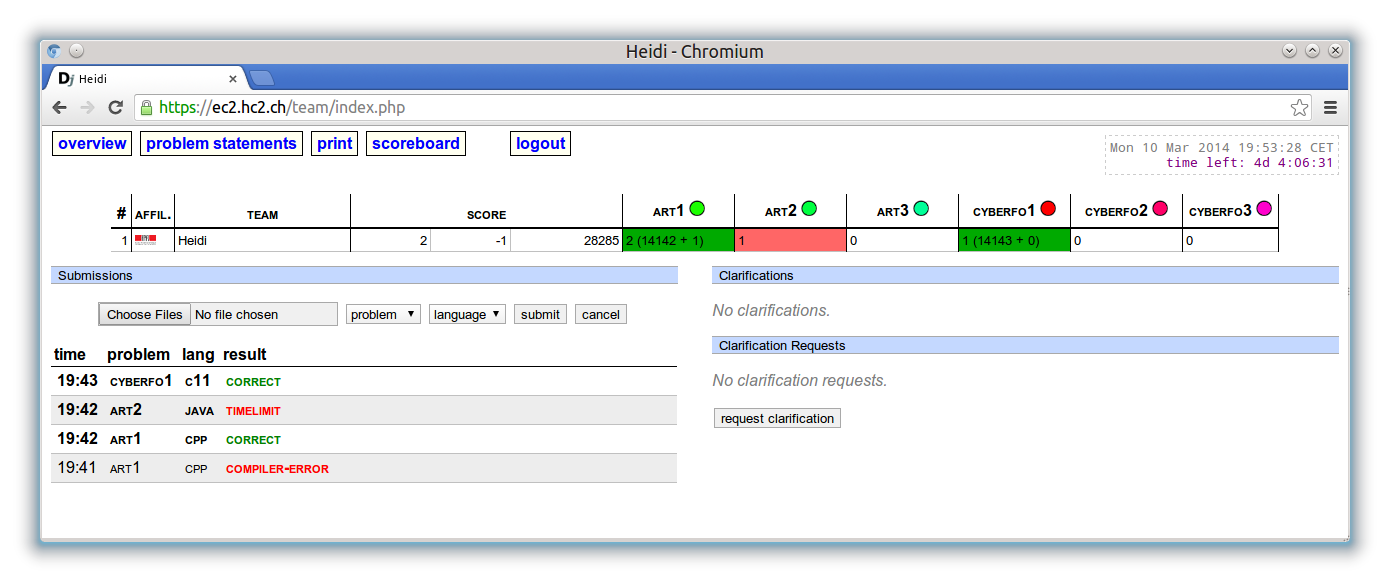
\includegraphics[width=0.9\textwidth]{overview.png}
\end{center}
\vskip -2 em
\caption{The team web interface overview page.}
\label{fig:overview}

\begin{center}
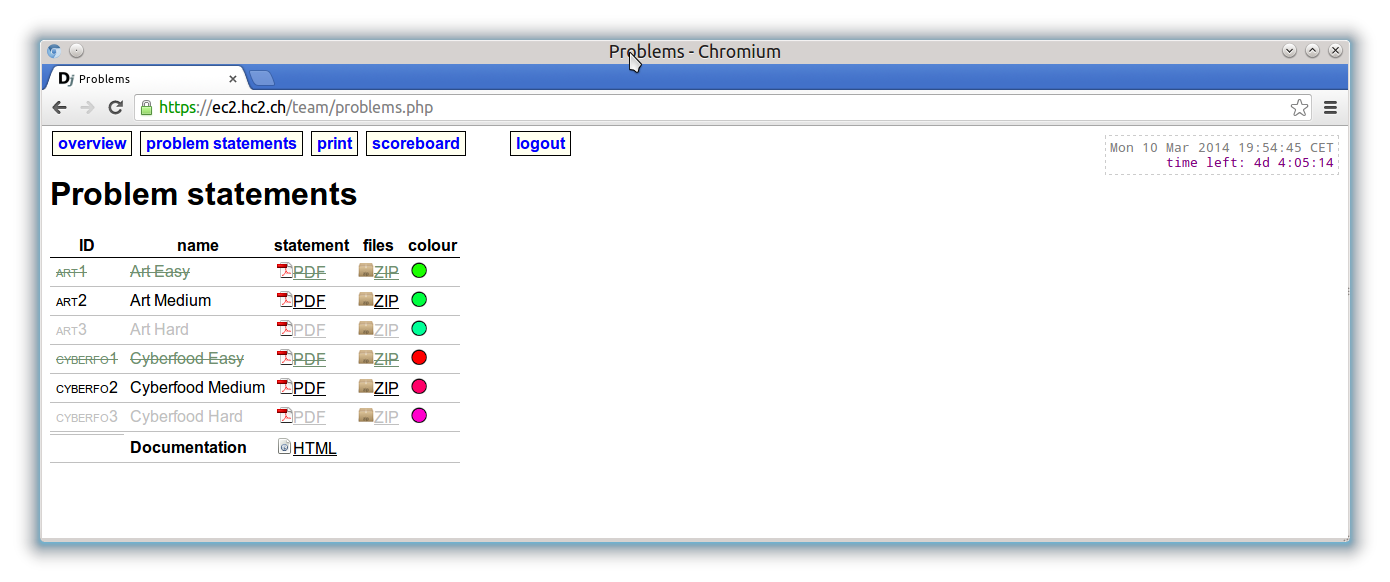
\includegraphics[width=0.9\textwidth]{statements.png}
\end{center}
\vskip -2 em
\caption{The problem statements page.}
\label{fig:statements}

\begin{center}
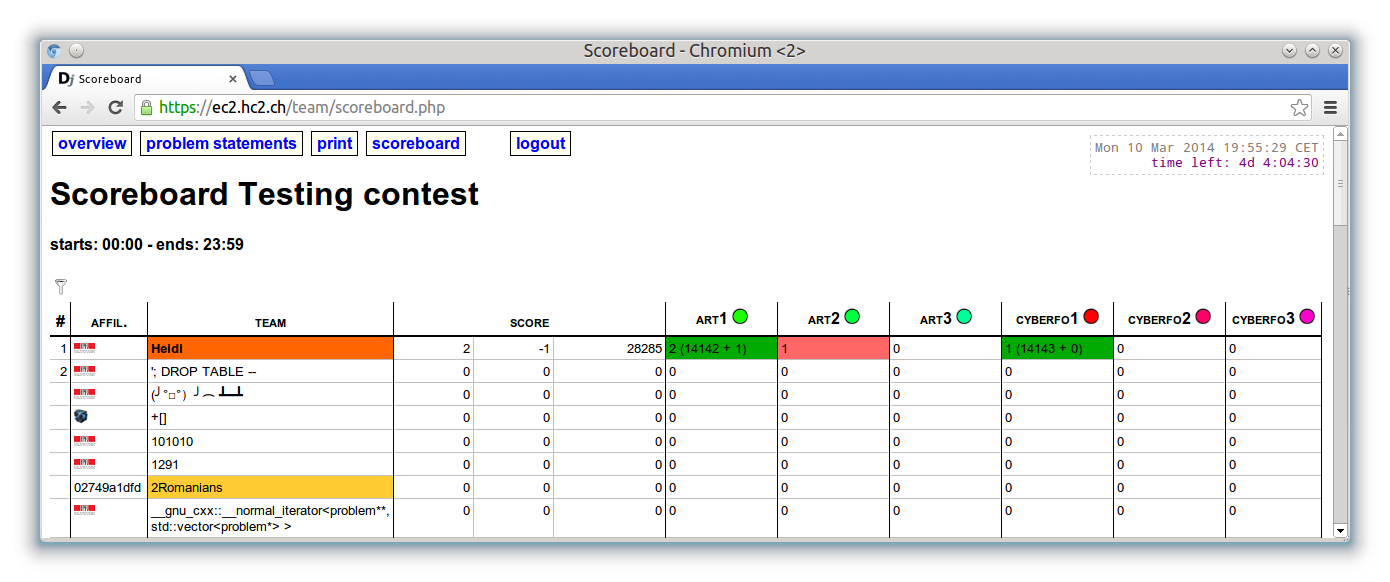
\includegraphics[width=0.9\textwidth]{ranking.png}
\end{center}
\vskip -2 em
\caption{The scoreboard webpage.}
\label{fig:ranking}
\end{figure*}


\paragraph{Problem statements and supporting material.}
The problem statements and supporting material are available
on the ``Problem statements'' tab of your team page.
Note that certain problems are greyed out: you will not be
able to see the statements for these until you solved
the problem above that one.
See Figure \ref{fig:statements}.

\paragraph{Reading and writing.}
Solutions have to read all input from `standard in' and write all
output to `standard out' (also known as console). You will never have
to open (other) files. See Section~\ref{codeexamples} for some
examples. Java users: keep in mind that java.util.Scanner might
be too slow for large input files.

Java, Scala: please stay in the default package, i.e., don't use the \texttt{package} keyword.


\paragraph{Compiling and testing your solution.}
Use the following commands to compile and test your code (replace the \textbf{bold} parts):
\begin{center}
\begin{tabular}{l|p{5cm}|p{7cm}}
C&hc2-compile \textbf{prob1}.c &hc2-run \textbf{prob1}.c $<$ \textbf{01}.in\\
C++11&hc2-compile \textbf{prob1}.cpp &hc2-run \textbf{prob1}.cpp $<$ \textbf{01}.in\\
C++98&hc2-compile \textbf{prob1}.c98 &hc2-run \textbf{prob1}.c98 $<$ \textbf{01}.in\\
Java&hc2-compile \textbf{Prob1}.java &hc2-run \textbf{Prob1}.java $<$ \textbf{01}.in\\
Scala&hc2-compile \textbf{Prob1}.scala &hc2-run \textbf{Prob1}.scala $<$ \textbf{01}.in\\
Python 2&hc2-compile \textbf{prob1}.py &hc2-run \textbf{prob1}.py $<$ \textbf{01}.in\\
Python 3&hc2-compile \textbf{prob1}.py3 &hc2-run \textbf{prob1}.py3 $<$ \textbf{01}.in\\
Ruby&hc2-compile \textbf{prob1}.rb &hc2-run \textbf{prob1}.rb $<$ \textbf{01}.in\\
Text&hc2-compile \textbf{prob1}.txt &hc2-run \textbf{prob1}.txt $<$ \textbf{01}.in\\
\end{tabular}
\end{center}

\paragraph{Submitting solutions.}
From your team ``Overview'' page,
\url{https://ec2.hc2.ch/team},
click ``Select file...'' in the left column and select the file
you want to submit. By default, the problem is selected from the
base of the filename and the language from the extension.
See Figure \ref{fig:overview}.

For some problems, we ask you to submit a text file containing the solution.

\paragraph{Printing.}
You can print files on the ``Print'' tab of your team page.
Select the file you want to print and click on ``print code''.
Your printout will be delivered to your workstation,
\emph{please do not fetch it yourself}. For the
environment's sake, please exercise moderation in
using this feature.


\clearpage
\section{Submitting solutions}
\label{sec:submit}
Solutions must be submitted through Domjudge's web interface
at \url{https://ec2.hc2.ch/team}.
If this is the first time you go to that page
you will need to login with your username and password (which will be
distributed shortly before the contest). If you have trouble accessing
the interface, please raise your hand and wait for an organizer to come
and assist you.

In the left column click ``Select file...'' to select the
file for submission. Domjudge will try to determine the
problem and language from the base and extension of the filename,
respectively. Otherwise, select the appropriate values.

After you hit the ``submit'' button and confirm your submission,
you will be redirected back to your submission list page. On this
page, a message will be displayed that your submission was
successful and the submission should be present in the list.
An error message will be displayed if something went wrong.

\section{Viewing the results of submissions}
The left column of your team web page shows an overview of
your submissions. It contains all the relevant
information: submission time, programming language, problem
and status. The address of your team page is
\url{https://ec2.hc2.ch/team}.

The top of the page shows your team's row in the scoreboard:
your position and which problems you attempted and solved.
Via the menu you can view the public scoreboard page with
the score from all the teams. One hour before the end of
the contest however, the scoreboard will be ``frozen'';
the full scoreboard view will not be updated anymore, but your
team row will. Your team's rank will be displayed as ``?''.

\subsection{Possible results}
A submission can have the following results:

\begin{center}
\begin{longtable}{|l|p{12.5cm}|}
\hline
\textbf{Verdict} &
\textbf{Description}\\\hline
Correct &
Your program passed all tests: you solved this problem!\\\hline
Compiler-error &
There was an error when compiling your program. On the submission
details page you can inspect the exact error.
\\\hline
Timelimit &
Your program took longer that the maximum allowed time for this
problem. Therefore it has been aborted. This might indicate that
your program hangs in a loop or that your solution is not
efficient enough.\\\hline
Run-error &
% FIXME: exit code 0 is rather irrelevant for hc2, isn't it?
There was an error during the execution of your program. This
can have a lot of different causes like division by zero,
incorrectly addressing memory (e.g., by indexing arrays out of
bounds), trying to use more memory that the limits, etc.
Also check that your program exists with exit code 0!\\\hline
No-output&
Your program did not produce any output. This probably means your
program exited early.\\\hline
Wrong-answer&
The output you produced was incorrect. (Note that the judge will
ignore differences in whitespace in your output.)
\\\hline
Too-late&
Bummer, you submitted after the contest ended! Your submission
is stored, but will not be processed anymore.\\\hline
\end{longtable}
\end{center}

\bigskip

\section{Clarifications}
All communication with the jury is to be done with clarifications. These
can be found in the right column on your team page.
Both clarification replies from the jury and requests sent by you are
displayed there.

There is also a button to submit a new clarification request to the
jury. This request is only readable for the jury and they will
respond as soon as possible. Answers that are relevant for
everyone will be sent to everyone.

It is your responsibility to check the clarifications column regularly.

\section[How are submissions being judged?]{How are submissions being
judged?}
\subsection{Submitting solutions}
With the web interface, you can submit a solution to a problem to the
jury (see Section \ref{sec:submit}). Note that you have to submit the source code
of your program (and not a compiled program or the output of your
program, unless explicitly stated otherwise in the problem description).
There your program enters a queue, awaiting compilation, execution
and testing on one of the jury computers.

\subsection{Compilation}
Your program will be compiled on a jury computer running Ubuntu Linux
(64 bits).

The compilation commands are as follows:
\begin{center}
\begin{tabular}{l|p{14cm}}
C&
gcc -Wall -O2 -static -pipe -o \$DEST \$SOURCE -lm \\
C++11&
g++ -Wall -O2 -static -pipe -std=c++11 -o \$DEST -x c++ \$SOURCE \\
C++98&
g++ -Wall -O2 -static -pipe -o \$DEST -x c++ \$SOURCE \\
Java&
javac -d . \$SOURCE \\
Scala&
scalac \$SOURCE \\
Ruby&
ruby -c \$SOURCE \\
\end{tabular}
\end{center}
where \$SOURCE represents the file you submitted.
Python source code and text files are not compiled.

\subsection{Testing}
After your program has compiled successfully, it will be executed and
its answer compared to the answer of the jury. Before comparing the
output, the exit status of your program is checked: if your program
exits with a non-zero exit code, the verdict will be
``Run-error''. There are some restrictions during execution;
if your program violates these, it will also be aborted with
a ``Run-error''.

The command for executing Java and Scala programs is as follows:
\begin{center}
\begin{tabular}{l|p{14cm}}
Java&
java -Xrs -Xmx393216k \$MAINCLASS\\
Scala&
scala -J-Xrs -J-Xmx393216k \$MAINCLASS \\
\end{tabular}
\end{center}
where \$MAINCLASS is the name of the class containing the \texttt{main} method.

\subsection{Restrictions}
To prevent abuse, keep the jury system stable and give everyone clear
and equal environments, there are some restrictions to which all
submissions are subjected:

\begin{center}
\begin{longtable}{|l|p{12cm}|}
\hline
Compile time&
Compilation of your program may take no longer than 30
seconds. After that compilation will be aborted and the result will
be a compile error. In practice this should never give rise to
problems. Should this happen to a normal program, please inform the
jury right away.\\\hline
Source size&
The source code of your program may not exceed 256 kilobytes,
otherwise your submission will be rejected.\\\hline
Memory&
During execution of your program, there are 256 megabytes of
memory available (364 MB for Java and Scala). This is the total amount of memory (including
program code, statically and dynamically defined variables, stack,
$\dots$ --- The Java VM will not be counted however).
If your program tries to use more memory, it will
abort, resulting in a run error.
\\\hline
Program output&
You are not allowed to output more than 4 megabytes
on standard output and standard error, and will get a ``Run-error''
if you exceed this limit.\\\hline
Number of processes&
You are not supposed to create multiple processes (threads). This is
to no avail anyway, because we look at the cpu-time to determine the runtime of your program.
To increase stability of the jury system, there is a
maximum of 10 processes that can be run simultaneously (100 for Java/Scala)
(including processes that started your program).

People who have never programmed with multiple processes (or have
never heard of ``threads'') do not have to worry: a normal program
runs in one process.\\\hline
\end{longtable}
\end{center}

\subsection[Java/Scala class and package naming]{Java/Scala class and package naming}
Compilation of Java/Scala sources is somewhat complicated by the class
naming conventions used: there is no fixed entry point; any class can
contain a method \texttt{main}. Furthermore, a class declared
\texttt{public} must be located in an identically named file.

Please stay in the default package, i.e., don't use the \texttt{package} keyword.

\section{Printing}
You can request to print a file via the ``print'' tab on your team page.
We will deliver the printouts to your workstation, so please
don't fetch them yourselves. We ask you to be
reasonable in using this feature (judges may impose a quota to prevent
abuse).

\emph{We also ask that you do not print the problem statements
yourself. We will deliver a copy of the statements of any new
problems that become available after you have solved a problem.}

\section{Problem statements and support material}
The problem statements and supporting material are available
on the ``Problem statements'' tab of your team page.
For each problem, we provide you with the problem statement
as a PDF, as well as a ZIP archive containing the sample input and output
(for offline problems, also the actual input).

\section{Compiling and testing your solution}
You should use the following command lines to compile your program
(replacing the bold parts as appropriate):
\begin{center}
\begin{tabular}{l|p{14cm}}
C&
gcc -Wall -O2 -static -pipe -o \textbf{prob1} \textbf{prob1}.c -lm \\
C++11&
g++ -Wall -O2 -static -pipe -std=c++11 -o \textbf{prob1} -x c++ \textbf{prob1}.cpp \\
C++98&
g++ -Wall -O2 -static -pipe -o \textbf{prob1} -x c++ \textbf{prob1}.c98 \\
Java&
javac -d . \textbf{Prob1}.java\\
Scala&
scalac \textbf{Prob1}.scala\\
Python 2&
true\\
Python 3&
true\\
Ruby&
ruby -c \textbf{prob1}.rb\\
Text&
true\\
\end{tabular}
\end{center}
And the following to test your solution with the sample input \textbf{01}.in:
\begin{center}
\begin{tabular}{l|p{14cm}}
C&
./\textbf{prob1} $<$ \textbf{01}.in\\
C++11&
./\textbf{prob1} $<$ \textbf{01}.in\\
C++98&
./\textbf{prob1} $<$ \textbf{01}.in\\
Java&
java -Xrs -Xmx393216k \textbf{Prob1} $<$ \textbf{01}.in\\
Scala&
scala -J-Xrs -J-Xmx393216k \textbf{Prob1} $<$ \textbf{01}.in\\
Python 2&
python \textbf{prob1}.py $<$ \textbf{01}.in\\
Python 3&
python3 \textbf{prob1}.py3 $<$ \textbf{01}.in\\
Ruby&
ruby \textbf{prob1}.rb $<$ \textbf{01}.in\\
Text&
cat \textbf{prob1}.txt \\
\end{tabular}
\end{center}
Alternatively, you may use hc2-compile and hc2-run as explained on the first page.

\section{Ranking}
Teams are ranked by the total number of problems solved, where more points is better. This is the first number displayed in the ``score'' column of the scoreboard.

If teams tie after applying the previous rule, they are ranked by total number of penalities, where less penalities is better. For each problem that was solved on the $n$th attempt and
$t$ minutes after the start of the contest,
you will receive $(n-1)*20+t$ penalties.
This is the third number displayed in the ``score'' column.

\section{Easy-Medium-Hard progression}
At the beginning of the contest, only about one third of the problems will be available.
These are either standalone problems or so-called ``easy'' problems.
Once your team correctly solves an ``easy'' problem, the corresponding
``medium'' problem will become available. You will then be able to download the
problem statement and support material from the ``Problem statements'' page;
and a member of staff will bring you a printout of the problem statement.

When you solved a ``medium'' problem you will get access to the corresponding
``hard'' problem, and your team will receive a balloon.

You will also receive a balloon for solving a ``hard'' problem.

\section{C/C++/C++11/Java/Scala/Python/Ruby reference}
During the contest, you are allowed to access reference documents for C, C++, Java, Scala, Python 2, Python 3, and Ruby.
These provide you with references of the standard library of the
respective language.
Bookmarks has been created for that effect in your
web browser. Alternatively, you can type in the address
\url{http://doc.hc2.ch/} directly.

\section{Sample code}
\label{codeexamples}

In this section, we provide sample code to solve the following problem.
For each testcase, you are given two integers between 0 and $2^{30}-1$, and must output their sum and their difference.
The input file starts with an integer on a line by itself: the number of testcases.
Each testcase is on a line by itself, and contains two integers $a$ and $b$ separated by a single space.
For each testcase, output the integers $a+b$ and $a-b$ separated by a single space on a line by itself.

\begin{tabular}{|p{0.47\textwidth}|p{0.47\textwidth}|}
\hline
\textbf{Sample input} & \textbf{Sample output} \\
\hline
\verbatiminput{sample/01.in} &
\verbatiminput{sample/01.out} \\
\hline
\end{tabular}

\begin{tabular}{|p{0.47\textwidth}|p{0.47\textwidth}|}
\hline
\textbf{C} & \textbf{C++} \\
\hline
\verbatiminput{sample/sample.c}&
\verbatiminput{sample/sample.cpp}\\
\hline
\end{tabular}

\begin{tabular}{|p{0.965\textwidth}|}
\hline
\textbf{Ruby}\\
\hline
\verbatiminput{sample/sample.rb}\\
\hline
\end{tabular}


\begin{tabular}{|p{0.965\textwidth}|}
\hline
\textbf{Java}\\
\hline
\verbatiminput{sample/Sample.java}\\
\hline
\end{tabular}

\begin{tabular}{|p{0.965\textwidth}|}
\hline
\textbf{Scala}\\
\hline
\verbatiminput{sample/Sample.scala}\\
\hline
\end{tabular}

\begin{tabular}{|p{0.47\textwidth}|p{0.47\textwidth}|}
\hline
\textbf{Python 2} & \textbf{Python 3} \\
\hline
\verbatiminput{sample/sample.py}&
\verbatiminput{sample/sample.py3}\\
\hline
\end{tabular}

\end{document}
